\chapter{Results and Evaluation}
In order to assess the quality and performance of the proposed systems, we ran various qualitative and quantitative evaluations. The results of these evaluations are presented below.

\section{Hardware Limitations}
Our first plan was to run the Kalman filter on the Arduino itself. This proved challenging since the filter requires a lot of computation and we had doubts on the performance of Arduino with the filter on producing real time results. To that end, we implemented a simple Kalman filter that did not integrate all the aspects of the real filter in order to address the hardware limitation, which worked well but did not achieve our expected performance or results. The Arduino MKR 1010 is not designed for computationally intensive tasks like matrix multiplication. Small matrices (e.g., 3x3 or 4x4) can be handled reasonably, but as matrix sizes grow, performance drops significantly due to limited processing power and memory. NumPy uses highly optimized libraries like BLAS and LAPACK. These libraries leverage multi-threading, SIMD instructions, and efficient memory access patterns to maximize speed. The performance scales well with larger matrices.\cite{hellmers_2013_an} To that end, we decided to implement the complete Kalman filter in Python and we would transfer the sensor reading from the Arduino to a Laptop to process it.

\section{Positioning Systems}
\subsection{Wi-Fi Data Random Forest Regressor}
The Wi-Fi RFR model was evaluated on average error, max error, mean squared error, and R2 score in order to show various aspects of the model's behavior.
\begin{table}[h!]
\centering
\caption{Error Metrics for Test and Unseen Sets}
\label{tab:error_metrics}
\begin{tabular}{l c c} % Left, Center, Center alignment
\toprule
\textbf{Metric}                  & \textbf{Test Set} & \textbf{Unseen Set} \\ 
\midrule
Average Error (m)                & 6.47              & 6.93                \\
Max Error (m)                    & 9.27              & 11.33               \\
Mean Squared Error (m\textsuperscript{2}) & 43.9              & 49.7                \\
R\textsuperscript{2} Score       & 0.536             & -                   \\ 
\bottomrule
\end{tabular}
\end{table}

A qualitative sample of the RFR model running on a single data sequence is seen below, showing the Wi-Fi model's predictions in orange, and the ground truth positions in blue.
\begin{figure}[h] 
	\centering 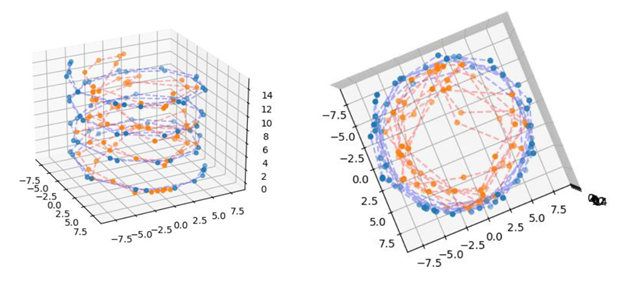
\includegraphics[height=4cm]{./images/wifirf.png}
	\caption{An example of the Wi-Fi RFR Model's predictions (orange) and  the ground truth path (blue).}
\end{figure}

\subsection{Kalman Filtering Schemes}
In the evaluation of the positioning system, three main metrics were used: the absolute trajectory error (ATE), relative trajectory error (RTE), and the average error. \cite{rtabmap, yan_2019_ronin} The implemented evaluations were implemented with a linear interpolation system, in order to be able to evaluate the metrics over two signals with different sample times.

\begin{table}[h!]
\centering
\caption{Trajectory and Average Errors Using Different Methods}
\label{tab:trajectory_errors}
\setlength{\tabcolsep}{3pt} % Adjust column spacing
\small % Reduce font size slightly to fit content
\begin{tabularx}{\columnwidth}{l X X X} % X columns for auto-adjust
\toprule
\textbf{Metric} & \textbf{Pressure Only} & 
\textbf{\centering Kalman Fusing Accelerometer and Pressure} & 
\textbf{Kalman with Wi-Fi Data} \\ 
\midrule
ATE (m) & 3.13 & 3.13 & 5.49 \\
RTE (m) & 2.81 & 2.80 & 2.87 \\
Average Error (m)             & 2.14 & 2.14 & 4.06 \\
\bottomrule
\end{tabularx}
\end{table}

\section{Orientation Estimation System}
In our evaluation of the orientation system, a preprocessing step was conducted in order to improve the synchronization of the ground truth and measured data. A cross correlation was calculated between the two signals and used to determine an optimal time shift between the two signals. Even with the rough synchronization applied during data collection, the cross correlation was still able to detect a time shift, which was accounted for in this evaluation.

\begin{figure}[h] 
	\centering 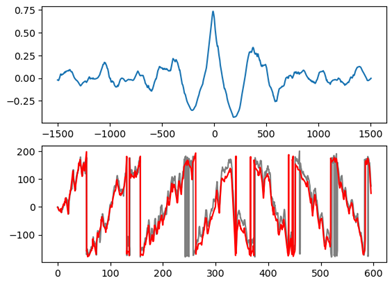
\includegraphics[height=4cm]{./images/crosscorrel.png}
	\caption{The results of the cross correlation of the ground truth and measured rotations (top) and the shifted data (red) after the delay was calculated (bottom).}
\end{figure}

\begin{table}[h!]
\centering
\caption{Error Metrics in Degrees}
\label{tab:single_value_metrics}
\setlength{\tabcolsep}{36pt} % Adjust column spacing
\small % Reduce font size
\begin{tabularx}{\columnwidth}{l c} % Left-aligned and center columns
\toprule
\textbf{Metric}      & \textbf{Value (\textdegree \ )} \\ 
\midrule
Median Error         & 28   \\
Average Error        & 35   \\
Max Error            & 168  \\ 
\bottomrule
\end{tabularx}
\end{table}

\begin{table}[h!]
\centering
\caption{Error Metrics for Roll, Pitch, and Yaw}
\label{tab:roll_pitch_yaw_errors}
\setlength{\tabcolsep}{10pt} % Adjust column spacing
\small % Reduce font size
\begin{tabularx}{\columnwidth}{l c c c} % Left and center columns
\toprule
\textbf{Metric}      & \textbf{Roll (\textdegree \ )} & \textbf{Pitch (\textdegree \ )} & \textbf{Yaw (\textdegree \ )} \\ 
\midrule
Median Error         & 27.4                   & 3.59                    & 2.42                  \\
Average Error        & 33.96                  & 3.85                    & 2.78                  \\
Max Error            & 168.36                 & 13.97                   & 11.67                 \\ 
\bottomrule
\end{tabularx}
\end{table}

Furthermore, a qualitative sample of a single sequence is shown below. In this sequence, the heading (roll) is represented by the red signals, and the pitch and yaw are represented as the blue and gray signals.

\begin{figure}[h] 
	\centering 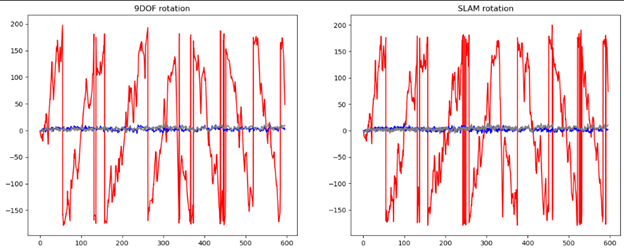
\includegraphics[height=3cm]{./images/rotations.png}
	\caption{The measured (left) and ground truth (right) rotation values with heading, pitch, and yaw in red, gray, blue respectively.}
\end{figure}


